\section{Case Study: Cloud-based Path Following Controller}
\label{sec:case_study}
For communication latency modeling, we initially adopted an analytical model approach inspired from the Mobile Cloud Computing area. However, we realized that the analytical model approach was inadequate to capture the mobility aspects of the vehicles and lacks the ability to specify accurate communication link characteristics. So, we utilized the NS-3 LTE library \cite{ref:ns3_lte} to simulate the communication channel and measure latency using UDP application traffic. We had used the measured latency values in a path following control system in Matlab and studied the behavior of the system in different scenarios and under varying network conditions.

\subsection{Communication channel modeling using NS-3 LTE library}
\label{sec:ns3_lte}
The simulation setup in NS-3 includes one base station (aka eNB node) and constant velocity mobility model for the vehicles. Since we used LTE communication technology, we generated two distinct categories of traffic – one related to the control application and another video streaming traffic. The traffic flow in the former category is bidirectional whereas the entertainment traffic is unidirectional (from streaming servers to the end users in vehicles). The simulation setup is shown in Figure \ref{fig:NS3-SETUP}. 
\begin{figure}
%\hspace{0.2in}
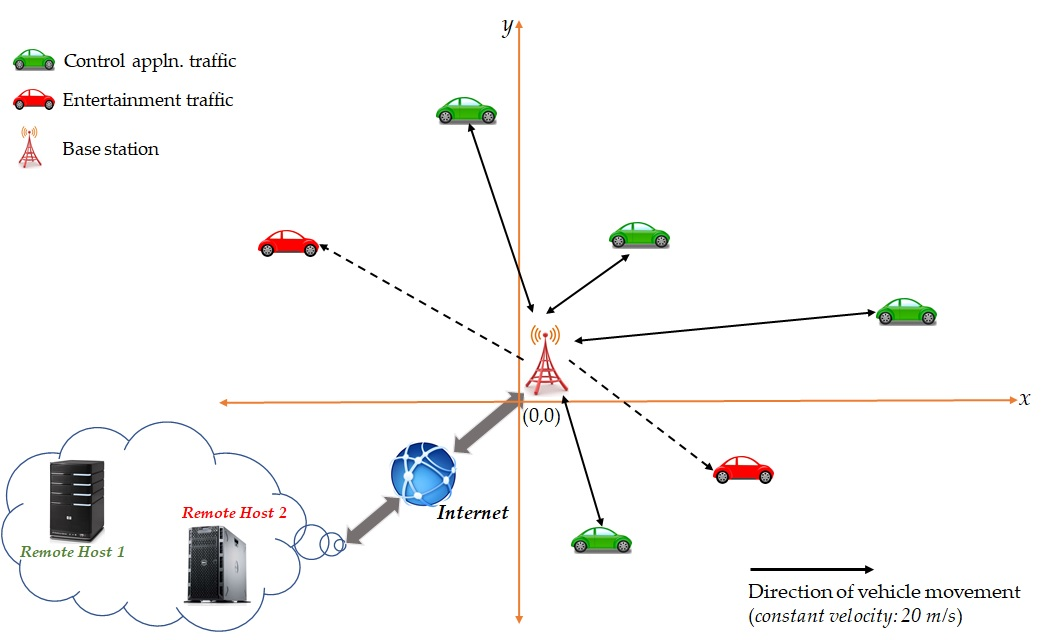
\includegraphics[width=3.5in,height=2.5in]{ns3_setup.jpg}
 \caption{Communication channel simulation setup  \label{fig:NS3-SETUP}}
\end{figure}

The downlink and uplink frequency bands of the cell are set to 2110 and 1710 MHz, respectively. The transmission power of the eNB node and the vehicle nodes is set to 40 and 20 dBm, respectively. In our simulation, Proportional Fair MAC Scheduler and Friis path loss model is used. The transmission method between the eNB node and vehicles is a single-hop unicast. Two distinct types of applications are configured on each remote host – an UDP Echo application on Remote Host 1 and a packet generator application on Remote Host 2. 

The control application traffic constitutes 80\% of the total traffic and the remaining 20\% is the entertainment traffic (1024 B packet every 20 ms). The packet size of the control application traffic transmitted by all but one vehicles is in the range of 128 to 2048 B every 20 ms. The remaining one vehicle, for which we are measuring the latency values, transmits 512 B packet every 20 ms. Table \ref{tab:ns3} shows the latency values obtained by varying number of vehicles and the network bandwidth. The latency values noted is an average of 10 runs for the vehicle the that transmits 512 B
packets every 20 ms. 

\begin{table}[ht]
\centering
\begin{tabular}{|l|c|c|c|c|c|}\hline
\theadfont\diagbox[width=11em]{{\bf Bandwidth}}{{\bf \# vehicles}}&
\thead{15}&\thead{30}&\thead{45}&\thead{60}&\thead{75}\\    \hline
5 MHz & 51.44 & 52.09  & 52.92 & 99.49  & 100.66\\
\hline
10 MHz & 37.28  & 42.01 & 42.1 & 68.49 & 89.38\\
\hline
\end{tabular}
\bigskip
\caption{Data transfer latency (ms)}
\label{tab:ns3}
\end{table} 

\subsection{Path following controller simulation in MATLAB}
\label{sec:matlab_sim}
We had chosen the pure pursuit controller algorithm that is available in the Robotic Systems Toolbox in Matlab \cite{ref:matlab_rst}. The sampling interval for the pure pursuit controller meets some of the offloading constraints specified in Section \ref{sec:Off_Ctlr} and hence determined as a suitable candidate to offload the computation to the cloud. 

The pure pursuit controller basically implements a path tracking algorithm that keeps track of and controls the robot’s movements along the path. The path between a source and destination is comprised of a set of waypoints (or intermediate [x y] coordinates). The fundamental operation in the controller is the computation of linear and angular velocities for the next control step based on the current pose of the robot. The pose is specified as [x, y, theta], where (x, y) represents a point in the reference coordinate system and “theta” represents the heading angle of the robot. 

In this work, we have extended the static waypoint generation and path following controller code (in \cite{ref:matlab_rst}) to dynamically generate waypoints using purely on-board or remote cloud resources. The other contribution is the simulation of failure scenarios such as network connectivity loss and large delays and demonstrate switching between local and cloud resources for waypoint generation. The cloud-based waypoint generation factors in the most up-to-date information about the constantly changing road conditions and hence can compute a more efficient path for the robot. 

In our work, we adopt a primitive approach for waypoint generation. We assume that the robot is operating in an environment where from any given point, there are three potential directions – namely, vertical, horizontal, or diagonal -- the robot can move on. Each potential direction has a weight associated with it that captures the “quality” of the path (e.g., if a path has a pothole or stalled traffic, it will have less weight and hence deemed as a low-quality path). The primitive waypoint generation algorithm always picks the path with the highest quality. In the local-only waypoint generation approach we assume that the weights remain static or change at much lower frequency compared to cloud (due to the large overhead incurred in V2V communication, for example). Therefore, the local-only approach might yield a path between source and destination that incurs larger distance, more time, or both. 

The first set of results shown in Figure \ref{fig:PF_A_B} demonstrates the differences in path computed fully on-board (a) and upfront (without factoring in changes in the road conditions) and path computed fully in the cloud (b) that dynamically adjusts weights based on crowdsourced data. We can see that the fully remotely computed path incurs less distance and time. The noted time values are adjusted by multiplying it with the path weight. For the cloud computation part, we have used the communication latency values obtained for N=30 vehicle case in the NS-3 simulation.

\begin{figure}
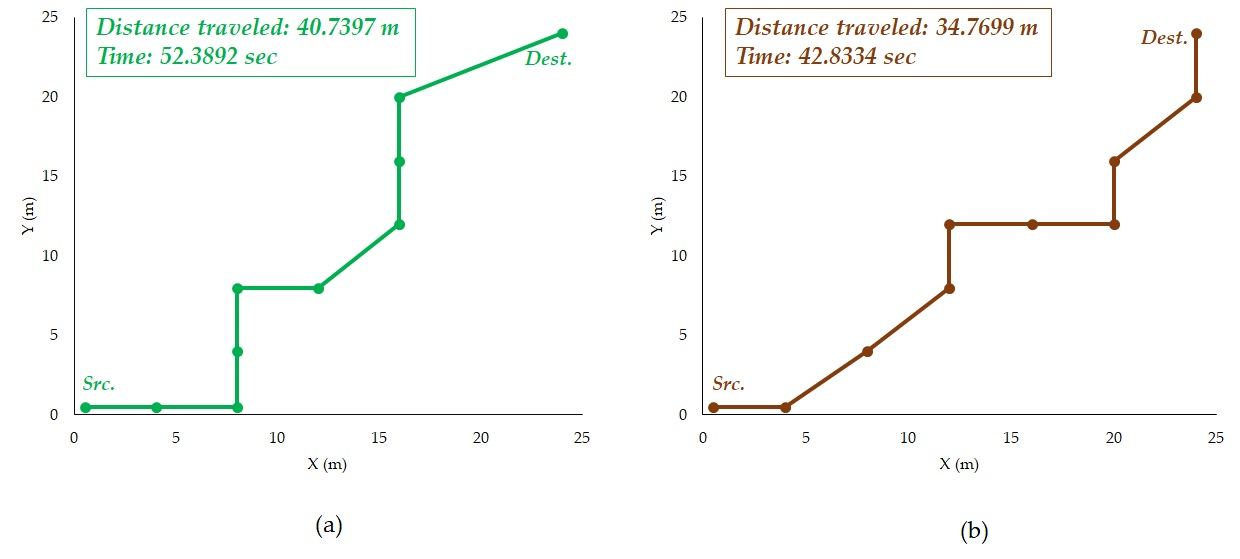
\includegraphics[width=3.5in,height=2.5in]{pf_a_b.jpg}
 \caption{Waypoint generation: (a) fully on-board without factoring in dynamically changing road conditions; (b) fully in the cloud using up-to-date data on current road conditions  \label{fig:PF_A_B}}
\end{figure}

The second set of results shown in Figure \ref{fig:PF_C} highlight the switching between local and remote resources in the presence of a network communication failure. It shows the impact of connectivity loss to the cloud server. When the connectivity loss is detected by the Network Performance Monitor component of the offloading controller (c.f.: Figure \ref{fig:OFF_CTLR}), the resource selector component chooses to leverage local resources for the next waypoint generation. Since the local knowledge is either static (or less frequently updated) compared to cloud, it results in a less efficient path than a purely cloud-based approach.

\begin{figure}
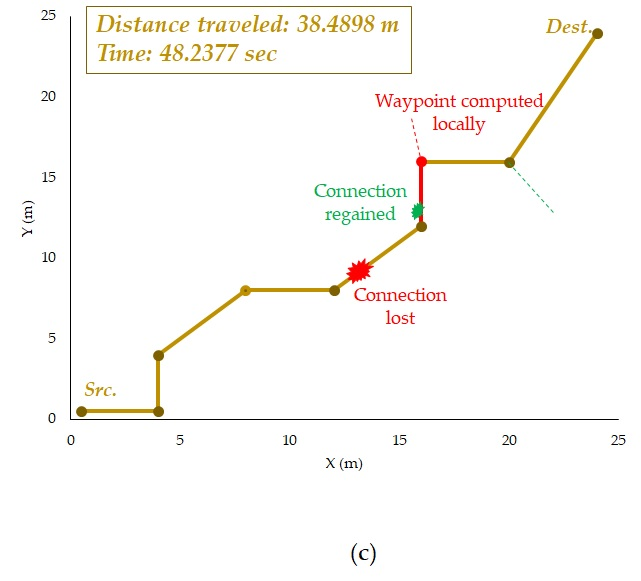
\includegraphics[width=2.5in,height=2.5in]{pf_c.jpg}
 \caption{Waypoint generation: (c) a scenario where both cloud and on-board resources are involved due to connectivity loss  \label{fig:PF_C}}
\end{figure}

Figure \ref{fig:PF_D_E} (d) shows a scenario where a request is originally forwarded to the cloud but the response hasn’t been received on time (say, due to temporary cloud resource outage). In this case, the timeout value for the request expires and the resource selector would choose to forward the request to the local resource (Note: here the timeout value is chosen based on the latency requirement to receive next waypoint specified in the Control Application Specification component in the offloading controller). Once the next waypoint from the cloud is received (after a large delay), the robotic controller would update its intermediate goal and starts moving towards that direction. 

\begin{figure}
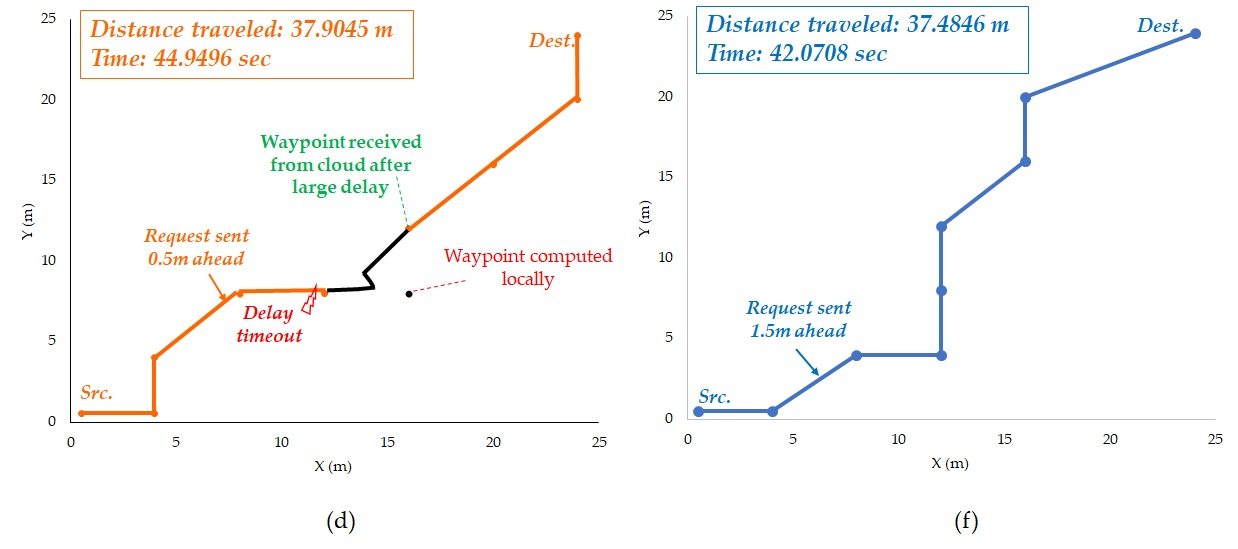
\includegraphics[width=3.5in,height=2.5in]{pf_d_e.jpg}
 \caption{Waypoint generation:  (d) a scenario where both cloud and on-board resources are involved due to large delay; (e) overcome transient large delays by requesting ahead of time  \label{fig:PF_D_E}}
\end{figure}

In Figure \ref{fig:PF_D_E} (d), the request for next waypoint is sent when the robot is 0.5 m ahead of the intermediate goal. One way to overcome large delay is to increase the distance at which the request for next waypoint is sent to the cloud. Figure \ref{fig:PF_D_E} (e) shows the performance results when the request is sent 1.5 m ahead of intermediate goal (as against 0.5 m ahead).

In this section, we have shown that a cloud-based path following controller improves the performance of the system compared a fully local resource based controller. Also, we have demonstrated the feasibility of switching between local and remote resources that effectively results in stable performance of the system despite a minor performance degradation.
